\chapter{Funções de Mão Única}
\label{cha:owf}

Nos Capítulos \ref{cha:cifras-de-fluxo}, \ref{cha:cifras-de-bloco} e \ref{cha:mac} mostramos que, sob certas condições, alguns sistemas de criptografia são seguros contra determinados tipos de ataque.
Essas condições incluem a existência de geradores de números pseudoaleatórios, funções pseudoaleatórias e permutações pseudoaleatórias.
Contudo, é importante destacar que, embora essas condições sejam amplamente aceitas, elas não foram provadas matematicamente, mas sim validadas por meio de experimentos práticos.

Neste capítulo, discutiremos por que não criamos sistemas que comprovadamente atendem a essas condições.
Para isso, apresentaremos um conceito fundamental:
a existência de funções de mão única, que são funções fáceis de calcular, mas difíceis de reverter.
Essas funções são a base para a segurança de sistemas criptográficos.
Além disso, explicaremos que provar a existência dessas funções seria o mesmo que provar que o problema P não é igual ao problema NP, um dos grandes desafios não resolvidos na matemática atual.

Este capítulo passará por vários dos principais resultados que já vimos e, assim, serve também como uma revisão do que foi apresentado até agora no livro.

Uma {\em Função de Mão Única} (FMU) $f: \{0,1\}^n \to \{0,1\}^n$ é uma função que tem duas características principais:

\begin{itemize}
\item[] {\em Fácil de computar}:
  Dado um valor $x$, calcular $f(x)$ é rápido (pode ser feito em tempo polinomial).
\item[] {\em Difícil de inverter}: Dado um resultado $y$, é muito difícil achar um $x$ que produza $y$ (encontrar uma pré-imagem não é algo que possa ser feito em tempo polinomial).
\end{itemize}

Em termos mais rigorosos, uma FMU é tal que, se um adversário eficiente (polinomial) recebe $y$, ele só é capaz de encontrar um $x$ que produza $y$ (ou seja, $f(x) = y$) com uma probabilidade desprezível \cite{Diffie76,Yao82}.

\begin{example}
  Uma candidata a função de mão é única é a seguinte função, onde $x$ e $y$ são números primos do mesmo tamanho:
  \begin{displaymath}
    f(x,y) := x \cdot y
  \end{displaymath}
  A dificuldade de inverter $f$ está a associada ao {\em problema da fatoração} que é considerado um problema difícil.

  Para certos grupos $G$ com gerador $g$ temos que a seguinte função $f$ é de mão única:
  \begin{displaymath}
    f_g(x) := g^x
  \end{displaymath}

A dificuldade de inverter esta função está associada ao {\em problema do logarítmo discreto}.
\end{example}

\section{Construindo um GNP}

Chamamos de {\em predicado de núcleo duro} um pequeno pedaço de informação, como um único bit, sobre $x$ que a função de mão única mantém escondido \cite{Blum84}.
Mesmo que o adversário conheça $y = f(x)$ ele não obtem informação adicional sobre esse bit.
Em outras palavras, a chance de o adversário polinomial adivinhar o bit é desprezivelmente maior do que meio.

\begin{theorem}[Goldreich-Levin]
  Assuma que uma função de mão única existe $f$.
  Então a função $g(x,r) = \langle f(x), r \rangle$ também é uma função de mão única e o predicado $\bigoplus_{i=1}^nx_ir_i$ é um predicado de núcleo duro para $g$ \cite{Goldreich89}.
\end{theorem}

Uma vez que conseguimos extrair um bit ``seguro'' de uma função de mão única, podemos usá-lo para criar um gerador de números pseudoaleatórios (GNP) que aumenta o tamanho da entrada em 1 bit.

\begin{theorem}
  Se $f$ uma função de mão única com um predicado de núcleo duro $nd$, então a função $f(s)$ concatenada com $nd(s)$ ($G(s) := f(s)||nd(s)$) é um GNP que expande em 1 bit o tamanho original de $s$.
\end{theorem}

Agora que podemos gerar um GNP que expande a entrada em 1 bit, podemos usá-lo para criar um GNP que expande a entrada em $p(n)$ bits, onde $p$ é qualquer polinômio e $n$ é o tamanho da entrada $s$.
Seja $G$ um GNP que expande a entrada em 1 bit, e construímos $G'$ da seguinte maneira:

Usamos $G$ para gerar $n+1$ bits.
O último bit gerado é usado como o primeiro bit da saída de $G'$, e os outros bits são usados como uma nova semente para $G$.
Repetimos esse processo até que $G'$ tenha gerado $p(n)$ bits.

Essa construção nos leva ao seguinte teorema:

\begin{theorem}
  Se existe um GNP que expande a entrada de tamanho $n$ em 1 bit, então, para qualquer polinômio $p$, existe um GNP que expande a entrada em $p(n)$ bits.
\end{theorem}

\begin{center}
\begin{tikzpicture}[node distance=1.5cm, auto]

% Primeira caixa s_0 = s0'
\node (s0) [draw, rectangle, minimum width=3cm, anchor=west] at (0,0) {$s_0' = s$};
\node at (-0.5, 0) { $s_0$ };

% Segunda caixa s_1
\node (s1) [draw, rectangle, minimum width=3cm, anchor=west] at (0,-2) {$s_1'$};
\node (delta1) [draw, dashed, rectangle, minimum width=1cm, anchor=west] at (3,-2) {$\delta_1'$};
\node at (-0.5, -2) { $s_1$ };

% Seta com rótulo
\path[draw,-latex] (s0) -- node[midway, right] {$G'$} (s1);

% Segunda caixa s_2
\node (s2) [draw, rectangle, minimum width=3cm, anchor=west] at (0,-4) {$s_2'$};
\node (delta1) [draw, dashed, rectangle, minimum width=2cm, anchor=west] at (3,-4) {$\delta_2'$};
\node at (-0.5, -4) { $s_2$ };

% Seta com rótulo
\path[draw,-latex] (s1) -- node[midway, right] {$G'$} (s2);

% Segunda caixa p
\node (p) [draw, rectangle, minimum width=3cm, anchor=west] at (0,-7) {$s_{p(n)}'$};
\node (delta1) [draw, dashed, rectangle, minimum width=4cm, anchor=west] at (3,-7) {$\delta_{p(n)}'$};
\node at (-0.5, -7) { $s_{p(n)}$ };

% Seta com rótulo
\path[draw,dashed,-latex] (s2) -- node[midway, right] {$G'$} (p);

\end{tikzpicture}
\end{center}

\section{Construindo uma FPA e um PPA}

Agora que entendemos como construir um GNP a partir de uma Função de Mão Única, vamos avançar para a construção de uma Função Pseudo-aleatória (FPA).
A construção de uma FPA é um passo fundamental em criptografia moderna, pois ela desempenha um papel central em vários protocolos de segurança.
Para construir uma FPA segura, precisaremos de um GNP que expanda o tamanho da entrada, ou seja, que gere uma saída com o dobro do tamanho da entrada original. 

Seja $G$ um GNP que dobra o tamanho da entrada $m$ e $k$ a chave que vamos usar para gerar a função $f_k$.
Primeiro, aplicamos $G$ à chave $k$.
Se o primeiro bit $m_1$ do bloco $m$ for 0, pegamos a primeira metade dos bits gerados (representado por $G_0$); se for 1, pegamos a segunda metade (representado por $G_1$).
Em seguida, aplicamos $G$ ao bloco escolhido e repetimos o processo para o próximo bit $m_2$ de $m$, continuando assim até processar todos os bits de $m$.
Ou seja:

\begin{displaymath}
f_k(m_1 \dots m_n) = G_{m_n}(\dots(G_{m_1}(k) \dots )
\end{displaymath}

\begin{theorem}[Yao]
  Se $G$ é um GNP que dobra o tamanho da entrada, então a construção acima gera uma FPA.
\end{theorem}

O diagrama abaixo representa um bloco de apenas dois bits:

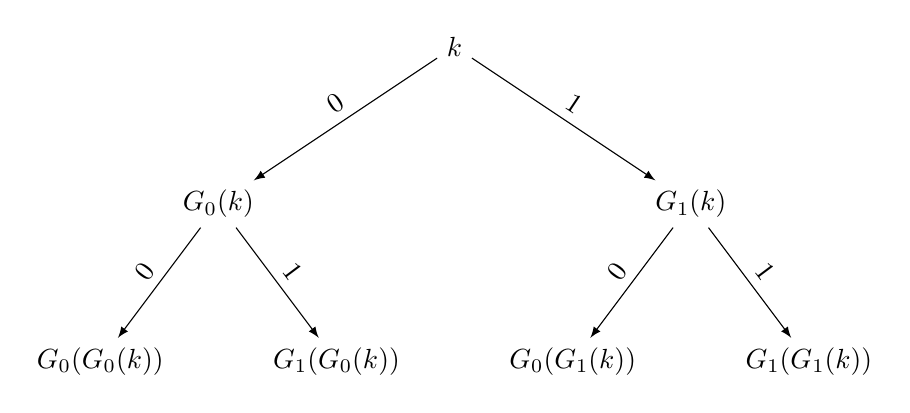
\begin{tikzpicture}
  [-latex]

  % Raiz da árvore
  \node (root) at (0,0) {$k$};
  
  % Primeira camada de nós
  \node (G0k) at (-3,-2) {$G_0(k)$};
  \node (G1k) at (3,-2) {$G_1(k)$};
  
  % Segunda camada de nós à esquerda
  \node (G00k) at (-4.5,-4) {$G_0(G_0(k))$};
  \node (G01k) at (-1.5,-4) {$G_1(G_0(k))$};
  
  % Segunda camada de nós à direita
  \node (G10k) at (1.5,-4) {$G_0(G_1(k))$};
  \node (G11k) at (4.5,-4) {$G_1(G_1(k))$};

  % Conectando nós da raiz para a primeira camada
  \draw (root) -- (G0k) node[midway, above, sloped] {0};
  \draw (root) -- (G1k) node[midway, above, sloped] {1};
  
  % Conectando nós da primeira camada para a segunda camada à esquerda
  \draw (G0k) -- (G00k) node[midway, above, sloped] {0};
  \draw (G0k) -- (G01k) node[midway, above, sloped] {1};
  
  % Conectando nós da primeira camada para a segunda camada à direita
  \draw (G1k) -- (G10k) node[midway, above, sloped] {0};
  \draw (G1k) -- (G11k) node[midway, above, sloped] {1};
\end{tikzpicture}

Para completar, a partir de uma FPA é possível construir uma PRP usando uma rede de Feistel como vimos no Capítulo \ref{cha:cifras-de-bloco}.
Para garantir uma PPA segura, precisamos de uma rede com pelo menos três passos em que cada passo use uma chave distinta.
\begin{displaymath}
  f_{k_1,k_2,k_3}^{(3)}(x) := Feistel_{f_{k_1},f_{k_2},f_{k_3}}(x)
\end{displaymath}
Lembrando que:

\begin{eqnarray*}
  Feistel_{f_1,\dots,f_n}(x) & := & L_nR_n\\
  L_i & := & R_{i-1}\\
  R_i & := & L_{i-1} \xor f_i(R_{i-1})
\end{eqnarray*}


\begin{theorem}
  Se $f$ é uma Função Pseudo-aleatória então $f^{(3)}$ é uma Permutação Pseudo-aleatória.
\end{theorem}

Resumindo, a existência de uma função de mão única é um ponto de partida na criptografia, pois ela nos permite construir Geradores de Números Pseudoaleatórios (GNP), Funções Pseudoaleatórias (FPA) e Permutações Pseudoaleatórias (PPA).
\begin{itemize}
\item No Capítulos \ref{cha:cifras-de-fluxo} vimos que a existência de um GNP é condição suficiente para construir um sistema seguro contra ataques ATC.
\item Nos Capítulos \ref{cha:cifras-de-bloco} e \ref{cha:mac} aprendemos que, se temos uma FPA, podemos construir sistemas de criptografia ainda mais robustos. Esses sistemas são seguros contra ataques mais avançados, como os ataques onde o atacante pode escolher textos para cifrar (ETP) ou até mesmo descriptografar (ETC).
  Além disso, a existência de uma FPA é suficiente para criar sistemas que garantem a autenticidade das mensagens seguro contra falsificação.
\end{itemize}

O teorema a seguir aborda a condição reversa, mostrando que a existência de uma função de mão única não só permite a criação de GNP, FPA e PPA, mas também que essa função de mão única é necessária para que essas construções existam:

\begin{theorem}
  Se existe um sistema seguro contra ataques {\em apenas contra o texto cifrado} (ATC) que protega uma mensagem duas vezes maior do que sua chave então existe uma função de mão única.
\end{theorem}
\begin{proof}
Para provar o teorema imagine que temos um sistema de criptografia que é seguro contra ataques ATC que consegue cifrar uma mensagem duas vezes maior do que a chave.

Queremos provar que, se tal sistema seguro existe, então também deve existir uma função de mão única.

Primeiro vamos sortear uma sequencia de bits aleatórios $r$ e então vamos construir uma função de mão única da seguinte forma:
\begin{displaymath}
  f(k, m, r) := E(k, m||r)||m
\end{displaymath}

Se um adversário polinomial for capaz de inverter $f$ então ele recupera $r$ e como $m$ está exposto, ele recupera a mensagem $m||r$.
Mas neste caso, o sistema de criptografia não seria seguro.
Como assumimos que o sistema é seguro, não deve ser possível inverter $f$.
\end{proof}

\section{Conclusão}

Acreditamos que certas funções são de mão única, ou seja, são fáceis de calcular, mas muito difíceis de inverter.
Essa crença é apoiada por muitos experimentos, mas ainda não temos uma prova matemática definitiva.

Agora, imagine que conseguíssemos provar que uma função $f$ é realmente de mão única.
Por definição, isso significa que podemos calcular $f(x)$ em tempo polinomial.
Além disso, se alguém nos der um valor $y$ e disser que $f^{-1}(x) = y$, podemos verificar isso rapidamente, testando se $f(y)=x$.

Em termos técnicos, isso significa que $f$ pode ser usada como um ``oráculo polinomial'' para verificar se uma solução está correta.
Isso coloca o problema de inverter $f$ na classe de problemas NP, que são aqueles problemas para os quais podemos verificar uma solução em tempo polinomial.

Por outro lado, a própria definição de função de mão única diz que inverter $f$ não pode ser feito de maneira polinomial.

A partir disso, podemos concluir que, se uma função de mão única existe, então a classe de problemas que podem ser resolvidos em tempo polinomial (P) é diferente da classe de problemas onde as soluções podem ser verificadas em tempo polinimal (NP).
Ou seja, provar que uma função é de mão única equivale a provar que P é diferente de NP.

Essa questão -- a relação entre os problemas P e NP -- é o maior problema em aberto na ciência da computação e um dos mais importantes em toda a matemática.
Dado que ainda não conseguimos resolver essa questão, nos contentamos em validar empiricamente que uma função é de mão única, que um gerador de números pseudoaleatórios é seguro, ou que uma permutação pseudoaleatória é segura.
A partir dessas validações, podemos então provar a segurança de diversos sistemas de criptografia, como fizemos nos capítulos anteriores.

O diagrama abaixo resume as construções que estudamos neste capítulo.
Se existir uma função de mão única, então é possível provar que existem GNPs (Geradores de Números Pseudoaleatórios), FPAs (Funções Pseudoaleatórias) e PPAs (Permutações Pseudoaleatórias) seguras.
Com esses elementos, poderíamos provar que cifras de fluxo e cifras de bloco podem ser usadas para criar sistemas seguros contra falsificação e todos os tipos de ataques que discutimos, incluindo ataques do tipo ETC.
No entanto, infelizmente, ainda não conseguimos provar a existência de funções de mão única.


\begin{center}
\begin{tikzpicture}[node distance=2cm, auto]

    % Nodos principais
    \node (owf) at (0,0) {FMU};
    \node (prg) at (3,0) {GNP};
    \node (prf) at (6,0) {FPA};
    \node (prp) at (9,0) {PPA};

    % Nodos de segurança
    \node (co) at (3,-2) {ATC};
    \node (cpa) at (6,-2) {ETP};
    \node (falsificacao) at (6,-4) {Falsificação};
    \node (cca) at (9,-2) {ETC};

    % Setas principais
    \path[-latex, draw] (owf) -- (prg);
    \path[-latex, draw] (prg) -- node[midway,above]{\tiny Yao} (prf);
    \path[-latex, draw] (prf) -- node[midway,above]{\tiny Feistel} (prp);

    % Setas pontilhadas
    \path[-latex, dashed, draw] (prg) -- (co);
    \path[-latex, dashed, draw] (prp) -- node[midway,right]{\tiny EBC} (cpa);
    \path[-latex, dashed, draw] (prf) -- node[midway,right]{\tiny Ctr} (cpa);
    \path[-latex, dashed, bend right=45, draw] (prf) to (falsificacao);
    \path[-latex, dashed, draw] (cpa) -- (cca);
    \path[-latex, dashed, draw] (falsificacao) -- (cca);

\end{tikzpicture}
\end{center}

\section{Exercícios}
%\label{sec:exercicios}

\begin{exercicio}
  Mostre que $f(x,y) = x \cdot y$ sem as restrições de que $x$ e $y$ sejam primos e do mesmo tamanho não é uma função de mão única.
\end{exercicio}


%\begin{exercicio}
%  Mostre um grupo cíclico com gerador $g$ (ver Capítulo \ref{cha:distribuicao-chaves}) em que $f_g(x) = g^x$ não é uma função de mão única.
%\end{exercicio}
